\icode{E-MD-MU-L3-2624-002}
（多选）
如图所示，质量为\(3m\)的物块\(A\)放在光滑的水平面上，轻绳的一端固定在物块\(A\)，另一端绕过两个光滑滑轮与质量为\(m\)的物块\(B\)相连，物块\(B\)与物块\(A\)紧挨在一起，两者接触面光滑，物块\(B\)一边下落一边随着物块\(A\)向右运动。重力加速度大小为\(g\)，滑轮质量不计，在物块\(B\)与地面接触之前，下列说法正确的是\paren[]

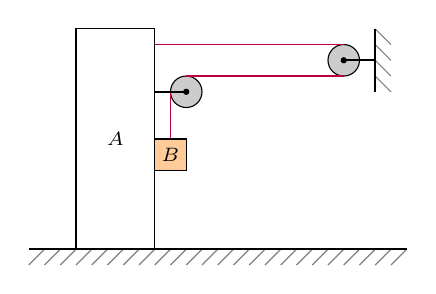
\begin{tikzpicture}[font=\scriptsize]
        \draw[fill=gray!40] (0,0) circle(.2) (2,.4) circle(.2);
        \draw[purple] (-.4,.6)--(2,.6) (2,.2)--(0,.2) (-.2,0)--(-.2,-.6);
        \draw[fill=orange!40] (-.4,-.6) rectangle(0,-1)node[midway]{\(B\)};
        \draw (-.4,.8) rectangle(-1.4,-2)node[midway]{\(A\)};
        \fill (0,0) circle(.04) (2,.4) circle(.04);
        \foreach \x in{-2,-1.8,...,2.6}
            \draw[gray] (\x,-2.2)--++(.2,.2);
        \foreach \y in{0,.2,...,.6}
            \draw[gray] (2.6,\y)--++(-.2,.2);
        \draw[thick] (2,.4)--(2.4,.4) (-.4,0)--(0,0) (-2,-2)--(2.8,-2) (2.4,0)--(2.4,.8);
\end{tikzpicture}
\begin{choices}
        \item 物块\(A\)、\(B\)的加速度大小相等
        \item 物块\(B\)的加速度大小等于\(\frac{\sqrt{5}}{4}g \)
        \item 物块\(A\)、\(B\)间的弹力大小等于\(\frac{1}{4}mg\)
        \item 绳子上的拉力大小等于\(\frac{\sqrt{5}}{2}g \)
\end{choices}
\begin{answer}
    BC\quad 提示：
\end{answer}